\chapter{Methods}
\label{chapter:Methods}



% Here starts the thesis with an introduction. Please use nice latex and bibtex entries \cite{latex}. Do not spend time on formating your thesis, but on its content. 
 
\section{Theorical Background}
There is no need for a latex introduction since there is plenty of literature out there.
\todo{ intro to approach}
 

\section{Notation and Symbols}
This section introduces the common mathematical notations and symbols used in this 
chapter.
Normal formatting such as $a$ and $A$ are used to indicate integers or real numbers while letters in scripts such $\mathcal{A}$ are reserved for sets. In addition, 
we use the symbols $\mathbb{R}$ for real numbers.
For 3D vectors, we use the uppercase bold letters $\mathbf{A}$ while for 2D vectors, 
we use the lowercase bold letters $\mathbf{a}$. If the vector if homogeneous, it will
be explicitly define; otherwise, the vector is assumed to be inhomogeneous. A vector
from point $A$ to $B$ is presented as $\overrightarrow{AB}$. Furthermore, matrices use
monospace font such as $\mathtt{A}$. If the dimension are specified such as $\mathtt{A}$$_{mxn}$,
$m$ would indicate the number of rows while $n$ indicates the numbers of columns.
Regardings accents, a hat on a vector such as $\hat{a}$ or $\hat{A}$ indicates the normalized
unit vector which means that $\hat{a}=\frac{a}{\|a\|}$ or $\hat{A}=\frac{A}{\|A\|}$.
A tilde on a 3D vector indicates that the last coordinate is removed; thus, the vector 
$A=(x,y,z)^T$ have $\hat{A}=(x,y)^T$  which is the projection of $A$ in the $xy$-axis,
while the vector with homogeneous coordinate $B=(x,y,z,1)^T$ have $\hat{B}=(x,y,z)^T$ 
which is the inhomogeneous coordinate of $B$. Lastly, a dot on top of variable indicates
the converged value of the variable after an algorithm is performed. For instances,
after using mean shift on $a_i$, it converges to a value $\dot{a}_i$

\section{Tracking Workflow and Theory}

The aim of this chapter is to define a basic workflow for the new tracking approach
and provide the reader with relevant literature review. The workflow will be divided
in to different functional processes. The requirements (Input) and the outcome (Output)
of each process will be defined. Based on these requirements relevant theorical concepts
will be discussed. The processes directly related to the problem statement will be 
discussed in detail, and a suitable approach will be suggested. The reader should
note that this chapter will provide only the overview of the theorical concepts, 
implementation specific details will be covered in Part \todo{some where} of the thesis.

\subsection{Basic Workflow}

\begin{figure}[ht]
\centering
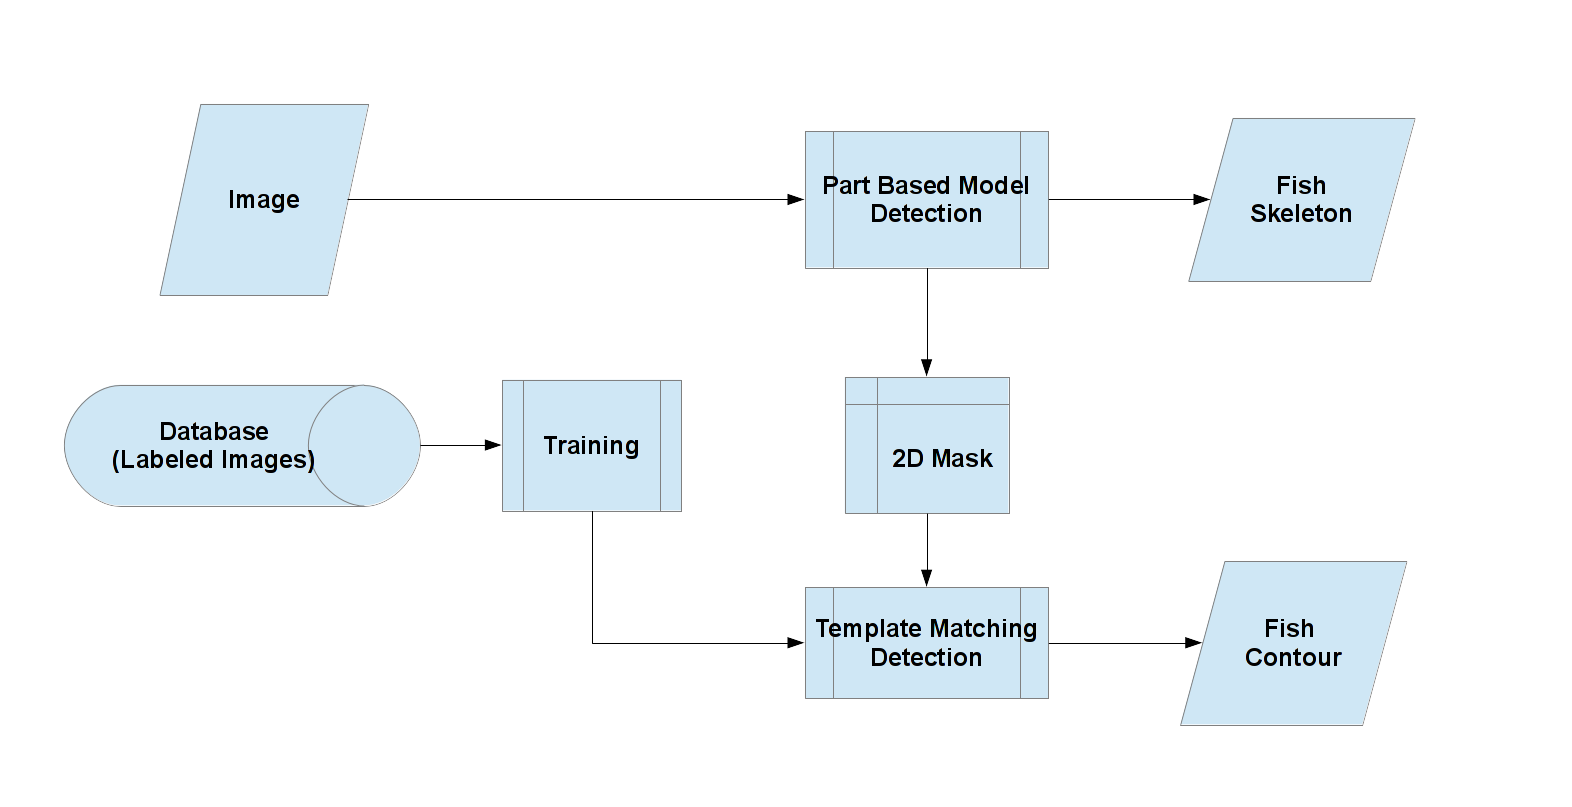
\includegraphics[scale=0.3]{flowchart_1}
\caption{A simplified workflow of the Detection process}
\label{fig:basicworkflow}
\end{figure}

\ref{fig:basicworkflow} shows the basic workflow of the detection process. The figure 
shows that once image is captured, it is supplied to the Part Based model detection 
process to extract 2D bounding boxes from the define part based fish model. Also from
this process can be extracted the skeleton of the fish, After 2D mask are generated, 
template detection matching process will take the 2D masked image and in those defined
areas will match the learned templates using the linemod algorithm propose in \citet{Hinterstoisser2012}. It is assumed that two detection process has been trained with the
proper labeled fish images in a offline procedure. A short introduction to the terms, processes and their functionalities is given below.

\begin{itemize}
\item \textit{Image}, this term refers to the two dimensional photographic image of the object
captured by the camera. It is given as a input for the detection workflow. The reader 
should note that the image provided to the workflow come from the underwater rig system
develop as part of the project.
which suggests that we are dealing with a deformable (articulated) object.
\item \textit{Database}, This term represents all the preprocessed information that 
is readily available to the detection workflow. This information includes details
regarding labeled data for training, trained model for Part Based detection process,
and trained model for template matching process.
\item \textit{2D Mask}, \todo{define}
\item \textit{Part Based Model Detection}, this term refers to a broad class of 
detection algorithms used on images, in which various parts of the image are used 
separately in order to determine if and where an object of interest exists. 
Amongst these methods a very popular one is the constellation model which refers 
to those schemes which seek to detect a small number of features and their relative 
positions to then determine whether or not the object of interest is present. 
\item \textit{Template Matching Detection}, This term refers to \todo{define}
\item \textit{Training}, \todo{define}
\item \textit{Fish skeleton}, \todo{define}
\item \textit{Fish Contour}, \todo{define}
\end{itemize}

\subsection{Part Based model Detection}
In this section will be discuss the method used to achieve the first task define in \ref{subsection:Basic Workflow}, analysing our target object, the fish, which can be 
model like a deformable object with one main deformation axis, the one define by the backbone, Most fish move by alternately contracting paired sets of muscles on either side of the backbone. These contractions form S-shaped curves that move down the body.
The pictorial structure framework arise as a feasible approach, which decomposes the appearance
of the objects into local part templates, together with geometric constraints on pairs of parts, often visualized as a spring. when parts are parametrized by pixel location and orientation, the resulting structure can model articulation. This has been 
the dominant approach for human pose estimation. For our problem comparing with Full-body pose estimation where many degrees of freedom has to be estimated, The fish is
a simplification due to the movement constraints, and also the absence of big limbs which are replace by small fins, those fins not vary greatly in appearance in compare with human limbs.
in the broad class of part based detection algorithm, the one propose by \citet{Ramanan2012} arise as the state of the arts, and is the one selected to be applied in
our problem.
\subsection{Model}
Let us write $I$ for a image, $l_i = (x,y)$ for the pixel location of part $i$ and $t_i$ for the mixture component of part $i$. We write $i$ $\in$  $\{1\dotsc K\}$, $l_i \in \{1\dotsc L\}$ and $t_i \in \{1\dotsc T\}$. we call $t_i$ the ``type" of part $i$.
\todo{adapt example} Our motivating examples of types include orientations of parts (e.g., a vertical versus horizontally oriented hand), but types may span out-of-plane
rotations (front-view head versus side-view head) or even semantic classes ( an open versus side-view head) or even semantic classes (an open versus closed hand). For notational
convenience, we define lack of subscript to indicate a set spanned by that subscript
(e,g,. $t=\{t1\dotsc t_K\}$. For simplicity, we define our model at a fixed scale; at test time we detect people of different sizes by searching over an image pyramid.

\textit{Co-occurrence model:} To score of a configuration of parts, we first 
define a compatibility function for part types that factors into a sum of local and pairwise scores:
\begin{equation}
S(t)=\sum_{i\in V} b_i^{t_i} + \sum_{ij\in E} b_{ij}^{t_i,t_j}
\end{equation}

The parameter $b_i^{t_i}$ favors particular type assignments for part $i$, while
the pairwise parameter $b_ij^{t_i,t_j}$ favors particular co-occurrences of part types.
For example, if part types correspond to orientations and part $i$ and $j$ are on the
same rigid limb, then  $b_ij^{t_i,t_j}$ would favor consistent orientation assignments.
Specifically,  $b_ij^{t_i,t_j}$ should be a large positive number for consistent
orientations $t_i$ and $t_j$, and a large negative number for inconsistent orientations
$t_i$ and $t_j$.

\textit{Rigidity:} we write $G = (V,E)$ for a (tree-structured) $K-node$ relational
graph whose edges specify which pairs of parts are constrained to have consistent
relations.Such a graph can still encode relations between distant parts through transitivity.
For example, our model can force a collection of parts to share the same orientation,
so long as the parts to share the same orientation, so long as the parts form a connected
$subtree$ of $G = (V,E)$. We use this property to model multiple parts on the torso.
Since co-occurrence parameters are learned, our model learns which collections of parts should be rigid.
We can now write the full score associated with a configuration of part types and positions:
\begin{equation}
\label{eq:rigidity}
S(t,l,t)=S(t) + \sum_{i\in V} \omega_i^{t_i} \dot \phi(I,l_i) + \sum_{ij\in E} \omega_{ij}^{t_i,t_j} \dot \psi(l_i - l_j)
\end{equation}

where $\phi(I,l_i)$ is a feature vector( e.g, HOG descriptor \citet{Dalal2005})
extracted from pixel location $l_i$ in image $I$. we write $\psi(l_i - l_j)=[dx\; dx^2\; dy\; dy^2]^T$, where $dx=x_i - x_j$ and $dy=y_i - y_j$, the relative location is defined
with respect to the pixel grid and not the orientation of part $i$ (as in classic 
articulated pictorial structures).

\textit{Appearance model:} The first sum in \ref{eq:rigidity} is an appearance model that computes the local score of placing a template $\omega_i^{t_i}$ for part $i$,
tuned for type $t_i$, at location $l_i$.

\textit{Deformation model:} The Second term can be interpreted as a \"switching\"
spring model that controls the relative placement of part $i$ and part $j$ by switching
 between a collection of springs. Each spring is tailored for a particular pair of 
 types $(t_i,t_j)$, and is parametrized by its rest location and rigidity, which are 
 encoded by $\omega_{ij}^{t_i, t_j}$.Our switching spring model encodes the dependende
 of local appearance on geometry, since different pairs of local mixtures are constrained
 to use different springs. Together with the co-occurrence term, it specifies an
 image-independent ``prior" over part locations and types.

 \subsection{Inference}




 \subsection{Learning}
 We assume a supervised learning paradigm. Given labeled positive examples ${I_n, l_n,t_n}$ 
and negative examples ${I_n}$, we will define a strcutured prediction objective function similar to those proposed in 



\section{Linemod}
There is no need for a latex introduction since there is plenty of literature out there.
process to extract